\documentclass[12pt]{article}
\usepackage[utf8]{inputenc}
\usepackage{amsmath}
\usepackage{color,lineno,setspace,multirow,kpfonts}
\usepackage{graphicx}
\usepackage[top=2.4cm,left=2.4cm,top=2.4cm,bottom=2.4cm,includefoot]{geometry}
\usepackage[style=bes]{biblatex}
\usepackage{rotating}

\bibliography{library, tim}

\begin{document}

\linenumbers 
\modulolinenumbers[1]

\textbf{Title:} A quantitative framework for network biogeography\\
% Alternative: The distribution of ecological interactions 
% Alternative: The biogeography of ecological interactions
% Alternative: Community macroecology: integrating species interactions and species distributions

\textbf{Authors:} Dominique Gravel$^{1,2,*}$, Timoth\'ee Poisot$^{1,2,3}$, Neo
Martinez$^{4}$, Jennifer Dunne$^{5}$, Jason Tylianakis$^{3}$, Nicolas
Mouquet$^{6}$, Daniel Stouffer$^{3}$ \\

1: Canada Research Chair in Biogeography and community ecology. D\'epartement de
biologie, chimie et g\'eographique, Universit\'e du Qu\'ebec \`a Rimouski, 300
All\'ee des Ursulines, Qu\'ebec, Canada. G5L 3A1.\\

2: Qu\'ebec Centre for Biodiversity Sciences\\

3: \\

4: \\

5: \\

6:\\

\textbf{Keywords:} networks, spatial ecology, co-occurrence, probability of interaction\\

\textbf{Words in the abstract:}  

\textbf{Words in the main text:}  

\textbf{Words in the legends:}   

\textbf{Figures:} 

\textbf{Tables:}         

\textbf{References:} 

\newpage
\doublespacing

%========================================================%
\section*{Abstract} 

\newpage
%========================================================%
\section*{Introduction}

Most ecology textbooks define the ecological community at \quote{the pool of
species occupying a given location at a given time, and the list of their
interactions} (ref to Morin?). Yet we oft forget the last part of this
definition, focusing on species and neglecting the way they interact.

\begin{itemize}
\item Network structure do vary in space in time. \\ 

\item We don't know yet to what extent interactions are varying with the
environment. \\

\item No theory to explain and interpret the meaning of network variation in space.
Current interpretation fo species turnover involves the effect of the
environment and stochasticity. \\

\item Objective: Propose a theoretical framework to understand and predict the
spatial and temporal variation in network structure.\\

\end{itemize}

\newpage
%========================================================%
\section*{A probabilistic representation of ecological networks}

Interaction networks do vary in space and time because any given pairwise
interaction could either occur or not at any particular location. We seek to
represent the probability an interaction between species $i$ and $j$ occurs at
location $y$. We consequently define $L_{ijy}$ as a stochastic variable taking a
value of 1 when an interaction occurs and are thus looking at the probabilty of
this event, $P(L_{ijy})$. There are several factors that could impact the
occurrence of an interaction and we will describe them below. But ultimately,
this probability depends on the spatial and temporal scale of observation. As
long as the interaction probability is not null, the probability of observing an
interaction will tend to 1 as the scale of observation increases. 
	  
The occurrence of an interaction requires the co-occurrence of species
$i$ and $j$. This argument might seem trivial at first, but the explicit
consideration of this condition in the probabilistic representation of
ecological networks will prove fundamental to understand their variation. We
thus define $X_{iy}$ as a stochastic variable representing the occurrence of a
species $i$ at location $y$, and similarly $X_{ijy}$ the co-occurrence of species
$i$ and $j$. The quantity we seek to understand is the probability of a joint
event:

%-----------------
\begin{equation}
	P(X_{iy},X_{jy},L_{ijy},)
\end{equation}
%-----------------

Which reads as the probability of observing species $i$, species $j$ and an
interaction between them. This probability could be further decomposed in two parts using the
product rule of probabilities:
%-----------------
\begin{equation}
	P(X_{iy},X_{jy},L_{ijy})=P(L_{ijy}|X_{iy},X_{jy},E_y)P(X_{iy},X_{jy}|E_y)
\end{equation}
%-----------------
We will refer to the left term as the metaweb. It is a conditional probability,
representing the probability that an interaction occurs if species $i$ and $j$
are co-occurring. The right term is the probability of observing the two species
co-occurring at location $y$.

The metaweb concept is making its way through the network litterature even
though it has never been formally and technically defined. It is usually
conceived as a network of interactions among species that could potentially
co-occur. It is usually represented by a binary matrix and thus
deterministically. Here we define it as the matrix of interaction probabilities
between co-occurring species. It thus represents potential interactions and
should therefore include interactions between species that never co-occurred but
are susceptible to. The problem with most representations of metawebs to date is
that the effect of co-occurrence is never factored out. The traditional approach
to build a metaweb is to cumulate observations across replicated networks. The
main problem with that approach is that the co-occurrence of rare species is
extremely unlikely and thus most often appear as an absence of interactions in
the metaweb. This approach is inappropriate because the observed co-occurrence
will have a strong signature on the evaluation of interactions. A rarefaction
analysis previously shown that interactions accumulate with the addition of
networks at a slower rate than species richness. It indicates that it is harder
to have a direct evaluation of interactions from observeration than it is to
evaluate species richness. If built from the observation of interactions, then
the only way to fill a metaweb is by running cafeteria experiments between all
pairs of species. Otherwise, the metaweb should be inferred using traits and
phylogenetic information. Most of the published metawebs are therefore
incomplete because of their sensitivity to sampling heterogeneity. We will come
back to the issue of evaluating the metaweb in the sections Example and Applications

There are many variants of the metaweb representing different hypotheses about
the origin of temporal and spatial variation in network structure (see the
explicit formulations at Table 1). First, the interaction could be 
deterministic instead of probabilistic. In other words, $P(L_{ijy}) = 1$ if
$X_{ijy} = 1$, and 0 otherwise. This representation of the metaweb is the one
mostly used so far, as soon as the species are found together they are assumed
to interact. It is also the only way to represent interactions when there is not
enough information available to evaluate the interaction probability. It should be a
reasonnable approximation when the sampling and inferrence scales are large
enough and that the only variation of networks considered arises from species
distribution. 

Ecological interactions could also depend on the environment.
Although it is not common to see a conditional representation of ecological
interactions, experimental studies of pairwise interactions revealing their
sensitivity to the environment are common (REF). For instance, it has been
documented that the predation risks of shorebirds do vary at the continental
scale, from the south to the north (REF). The effect of the environment on
interactions propagate up the community and influence network structure (REF).
Here the environment is considered in a very broad sense, as any factor
potentially influencing the probability of a pairwise interaction, provided that
the species co-occur. It thus includes both the biotic and the abiotic
components of environment. We note however that here the biotic environment
includes organisms that are not considered in the co-occurrence matrix.
Including a biotic component to the metaweb signifies that the pairwise
interaction is conditional on higher order interactions. An interaction modifier
occurs for instance when the predation risk by species $j$ might be impacted by
a parasite $k$ changing the behaviour of the prey $i$. We note that a
conditional probability approach could thus be used represent non-trophic
interactions into ecological networks (REF). This topic is however beyond the
scope of the current paper.

There are also variants to the co-occurrence matrix. Akin to the metaweb,
co-occurrence could be conditional or not. The simplest model relates
co-occurrence probability directly to the environment. In this situation there
is no underlying assumption about the ecological processes responsible for
co-occurrence. Alternatively, the co-occurrence probability could be a function
of the environment because of shared ecological requirements by the two species.
Species are independently distributed, but co-occur more often that expected by
chance alone because they are found on the same environments. We call this model
later neutral because species are specifically responding to the environment but
are independently distributed. Co-occurrence is then simply obtained by
multiplying the result of two independent and specific species distribution
models (SDM).

Finally, the co-occurrence probability itself could be dependent on ecological
interactions. Direct pairwise interactions such as competition, facilitation and
predation have long been studied for their impact on co-distribution. Second and
higher order interactions (e.g. trophic cascade) could also impact
co-occurrence. There is however currently no general theory on the expected
co-occurrence in complex ecological networks. For instance, we do not know how
far co-occurrence is not-random when going along the chain of indirect
interactions. Berlow(2009) shown previously that almost only first and second
order interactions do matter in ecological networks, but we don't know for
co-distribution. We neither know what is the sensitiviy to species richness: do
interactions tend to buffer each other? Generalizing knowledge aquired by the
study of small community modiles will require future research.

\newpage
%========================================================%
\section*{Interpretation: the integrated niche}

The niche concept is key to understand and predict species
distribution. Several attempts have been made to refresh it, but its main
usage still follows Hutchinson’s idea that species interactions restrict
the fundamental niche to a realized one, and ecologists haven't moved far past
the n-dimensional hypervolume formalism \parencite{Blonder2014}. Despite its
intuitive interpretation and translation into species distribution models,
the concept has been constantly criticized (Hardin, 1960; Peters, 1991;
Chase2003; Silvertown, 2004; Soberon, 2007) and several attempts have been
made to expand and reinforce it.

Part of the problem surrounding the definition of the niche has been
clarified with the distinction between Eltonian and Grinnellian definitions
(ChaseLeibold 2003). The Grinnellian dimension of the niche is the effect of
the environment on the demography of a species, while the Eltonian dimension
is the effect of a species on its environment \emph{sensu lato}.  % SNOB!
The Grinnellian niche is the most intuitive one to apply and is the conceptual
backbone of species distribution models. The Eltonian niche is well known
by community ecologists, but is trickier to turn into predictive models
\parencite{Devictor2010a}. Nonetheless, the development of the niche model
of food web structure (Williams2000) and its parameterization (Williams2010;
Gravel2013) made it more operational, although it has yet to be applied to
more than trophic interactions. 

While it is straigthforward to represent statistically the hyper volume where a species
occurs, it is much more challenging to account for ecological interactions.
Chase and Leibold (2003) attempted this representation in their definition:
\textit{[The niche is] the joint description of the environmental conditions
that allow a species to satisfy its minimum requirements so that the birth rate
of a local population is equal or greater than its death rate along with the set
of per capita effects of that species on these environmental conditions.} They
represented the niche graphically with zero-net growth isoclines (the Grinnelian
niche) and impact vectors (the Eltonian niche). While this representation has
been very influential in community ecology at the local scale, it remains
unpracticable at the biogeographical one.
% Why (or more to the point, what do we care about having the same definition at different scales?)?
The absence of any mathematical
representation of the niche that could easily be fit to ecological data perhaps
explain why biogeographers are still struggling to develop species distribution
models taking into account ecological interactions.

The key point to integrate dimensions of the niche is to represent the Eltonian niche into a Grinnelian space. 
- We do so by considering that the Eltonian niche is the hyper volume in the trait-space allowing an interaction. \\
- Doing so, we could project both niches in a plane and find the hypervolume where an interaction should occur (Fig. 2). \\
- This visual representation is parallel to the probabilistic definition of interaction probability. \\
- We propose that the metaweb is the Eltonian dimension of the niche, while the matrix of co-occurrence is the Grinnellian dimension. \\
- Feedbacks between dimensions occur through the inclusion of co-occurrence in the metaweb, and interactions in the co-occurrence matrix. \\
- This approach radically change the representation of the niche, putting species distribution and ecological interactions at the same level. \\
- Fitting the probabilistic model allows the evaluation of link distribution and species distribution models. \\
- Moreover, the integrated niche concept facilitates the formulation of species distribution models taking into account biotic interactions (see the section Applications) \\

 % TO BE COMPLETED

\newpage
%========================================================%
\section*{Example: network structure in different habitats}

In this section we provide an analysis illustrating the framework with an
empirical dataset of host-parasitoid networks. Data come from the study of
Tylianakis(2007) on the impacts of habitat modifications to the network
structure. The data consists of 48 networks with 4090 recorded interactions. The
advantage of replicated host-parasitoid networks is that usually every
interaction is observed, not inferred from a stationary metaweb. It thus allows
to evaluate interaction probability and to factor out the effect of
co-occurrence. Five habitats were sampled along a gradient of habitat
modification: forest, abandonned coffee agroforest, coffee agroforest, pasture
and rice culture. The metaweb consists of 9 parasitoids and kleptoparasites
(Hymenoptera: Eulophidae, Ichneumonidae, Leucospidae, Megachilidae and
Chrysididae; Dyptera: Bombyliidae) of 33 species of bees and wasps (Hymenoptera:
Apidae, Megachilidae, Mutilidae, Pompilidae, Sphecidae, Vespidae). The metaweb
is illustrated at Fig. 2, along with an example of one iteration of the metaweb.

Tylianakis (2007) investigated if habitat modification affects the structure of
these networks They found a significant impact of the habitat on their
structure, despite little variation in species richness. Increasing habitat
modification led to a higher parasitoid to host species ratio and a paraistoid
were also more specialized, thus impacting considerably vulnerability. A closer
inspection of the networks revealed that intensive agricultural systems were
dominated by a strong interaction and a specialization of the most abundanc
parasitoid. Although the discussion made clear that both the turnover in species
composition and the interaction probability changed with habitat modification,
it was not possible to partition these components.
 
We developped a R package (REF) to fit alternative formulations of the metaweb
and the co-occurrence matrix along an environmental gradient and run it to
re-interpret the data of Tylianaks (2007). The package provides a general
interface facilitating the development of different species and link
distribution models. It is also built to facilitate the interaction iwth the
Mangal database of ecological interactions (REF). The first step consists of
fitting a probablistic model from the observation of a pairwise interaction
(binary) and the environment (could be categorical or continuous) from the
subset of the data where the two species are co-occurring. In other words, it
fits the equation $P(L_{ijy}|X_{iy},X{jy},E_y)$ to the data where $X_{iy} = 1$
and $X_{iy} = 1$. Logistic regression was used and is currently programmed, but
alternative models could be used as well. The second steps consists of fitting a
a probabilistic model for co-occurrence over the whole dataset,
$P(X_{iy},X{jy}|E_y)$, independently of the observation of an interaction. The
two probabilities are then multiplied to obtain the probability of observing an
interaction (Eq. 2). We used this probability to compute the likelihood of each
observation ($\zeta(\theta|D) = P(L_{ijy},X_{iy},X_{jy})$ if $L_{ijy}=1$ and
$\zeta(\theta|D) = 1 - P(L_{ijy},X_{iy},X_{jy})$ otherwise). We then after
compare the models by their AIC.

We considered the gradient of habitat modification as a ordered categorical
variable and compared XX models (results are summarized at Table 2). Not
surprisingly the best model takes into account the effect of the environment on
both the metaweb and co-occurrence. What is most interesting are the comparisons
to the best model. First, we find that using a constant metaweb has a dramatic
impact on the fit of the model to the data (the AIC drops from X for model 1 to
X for model 2), indicating a strong effect of the environment on pairwise
interactions. Secondly, we find that the deterministic metaweb is the worst
model (model 3, AIC = ). This result indicate that the traditional appraoch to
consider that species interact as soon as they co-occur is definitely wrong.
Thirdly, we also find that using a constant co-occurrence does have a
significant impact on the model (the AIC drops to X, model 4), indicating there
is a non-random change in community composition with habitat modification. Taken
together, these two results better explain why network structured changed with
habitat modification, even though here we only used binary information about the
network structure. Another interesting result is that considering a neutral
co-occurrence did not impact much the fit of the modeel. The AIC drops to XX
with model 6, indicating that considering indepdenent SDMs yields similar
networks over this environmental gradient. This means that for this particular
dataset, ecological interactions does not have a strong impact on species
distribution since; a strong dependence of parasitoids to the host for instance
would have a occurrence probability higher than expected by chance, while a
repulsion would have had the opposite.

An important output of this analysis is a more explicit representation of the
uncertainty in the evaluation of the metaweb. We find that among the XX pairs of
host and parasitoids, XX did not co-occur. There were therefore many forbidden
links based on co-occurrence. These might never occur in reality, but we do not
know without doing extra experiments. Therefore, any analysis of the structure
of the metaweb would be inappropriate without filling those gaps. In addition to
specific experiments, the gaps could be filled with a trait-based approach,
using phylogenies or with a null hypothesis (e.g. the interaction probability is
equal to connectance computed on the observed interactions).

It is also possible to obtain for each pairwise interaction an estimate of the
uncertainty. Not surprisingly, the confidence interval is usually very high for
the estimation of a probability with a very small sample size. The standard
error on the evaluation of the interaction probability is provided along with
the metaweb at Fig. 3. It reveals that the uncertainty is very high for most
interactions, even if 48 networks were sampled. Such an approach could be used
to detect wich pairwise interaction requires additional sampling in order to
reduce the uncertainty to a manageable level.
  
\newpage
%========================================================%
\section*{Applications}

\subsection*{Network descriptors}

\subsection*{Partitionning beta diversity}

\subsection*{Guidance for empirical studies}

Ecological networks are known to be extremely sparse, \emph{i.e.} having far
more absences of interactions that they have interactions. These absences of
interactions, however, can come from different sources. The fact that unequal
sampling at the local scale can affect our understanding of network structure
is well documented \parencite{Martinez1999}. However, in a spatial context,
some interactions may be undocumented because the species involved have
never been observed in co-occurence. Although these are reported as a lack
of interactions, in actuality we cannot make inference about them seeing
that they have never been observed: it is possible that this interaction
may happen should the two species co-occur. A second category of absences
of interactions are those that are reported after multiple observations of
species co-occurence. However, so as to have a confidence in the fact that the
probability of an interaction is low, extensive sampling (that is, several
co-occurences) is needed. Generally, our confidence that the interaction
is indeed impossible will increase when the number of observations of the
species pair. Seeing that this is essentialy a Bernoulli process (what is
the probability that the species will interact given their presence), the
breadth of the confidence interval is expected to saturate after a fixed
number of observations, which can be set as a treshold above which a species
paier has been observed "often enough".

\subsection*{Null model testing}

\subsection*{Species \& link distribution models}

\newpage
%========================================================%
\section*{Conclusion}

\begin{itemize}
\item New research agenda\\

\item List of new questions \\
\end{itemize}

\newpage
%========================================================%
\section*{Acknowledgements}
This is tis a contribution to the Santa Fe Institute working group \emph{Networks over
ecological gradients}. DG received financial support from NSERC and Canada
Research Chair program. TP is supported by a MELS-FQRNT post-doctoral
fellowship. DG, TP, and DBS received financial support from the CIEE.
\newpage

%========================================================%
\printbibliography

\newpage
%========================================================%
\section*{Figure legends}

%------------------------
\subsection*{Figure 1}
\textbf{Non-random sampling of the metaweb}. The sampling of the metaweb is illustrated with a local interaction network from the Tylianakis et al (2007) dataset. Here the metaweb is simply the number of observed interactions over the 48 networks. Arrows points to species that are present in the local network \#34 (represented on the right).  

%------------------------
\subsection*{Figure 2}
\textbf{The integrated niche}.  The Grinnellian niche is the set of environmental conditions
where the intrinsic growth rate $r$ is positive (axioms i, ii \& iii).
Contingencies (axiom iv) such as disturbances and stochastic extinctions, in
conjunction with limited dispersal (axiom v), restrict species distribution to
the conditions where the colonization rate $c$ is larger than extinction rate
$e$. The Eltonian niche on the other dimension is represented by the set of
traits allowing species to interact (axiom viii). The red species is a predator
with a trophic position $n$, feeding on species whose niche is within a certain
range around the niche optimum $c$. The integrated niche combines the effects of
the environment and ecological interactions. The central square represents the
area where the joint probability of observing interactions and co-occurrence is
positive.

%------------------------
\subsection*{Figure 3}
\textbf{Uncertainty in the evaluation of the metaweb}. The inferred metaweb for the XX environment is represented (left), along with the uncertainty in the evaluation of the interaction probability (right). Note that the standard error for probabilities is not symetric and thus only the upper bound is represented. 

\newpage
%========================================================%
%------------------------
\subsection*{Figure 1}

\begin{figure}[ht!]
	\centering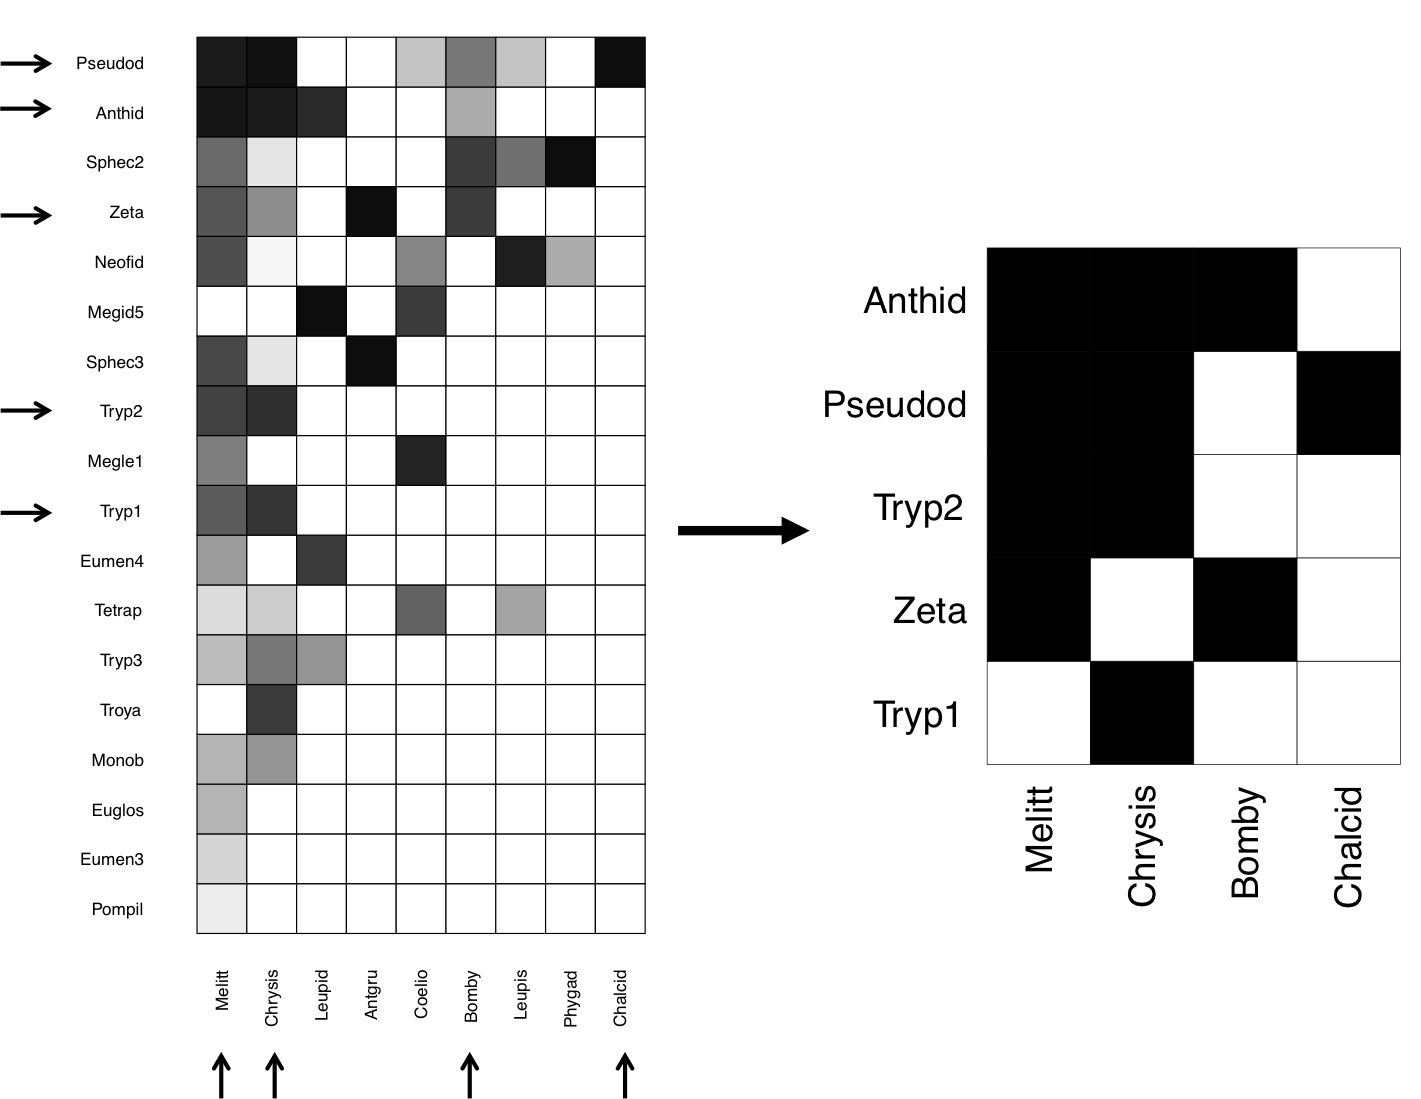
\includegraphics[width=0.8\textwidth]{sampling}
\end{figure}

\newpage

%------------------------
\subsection*{Figure 2}

\begin{figure}[ht!]
	\centering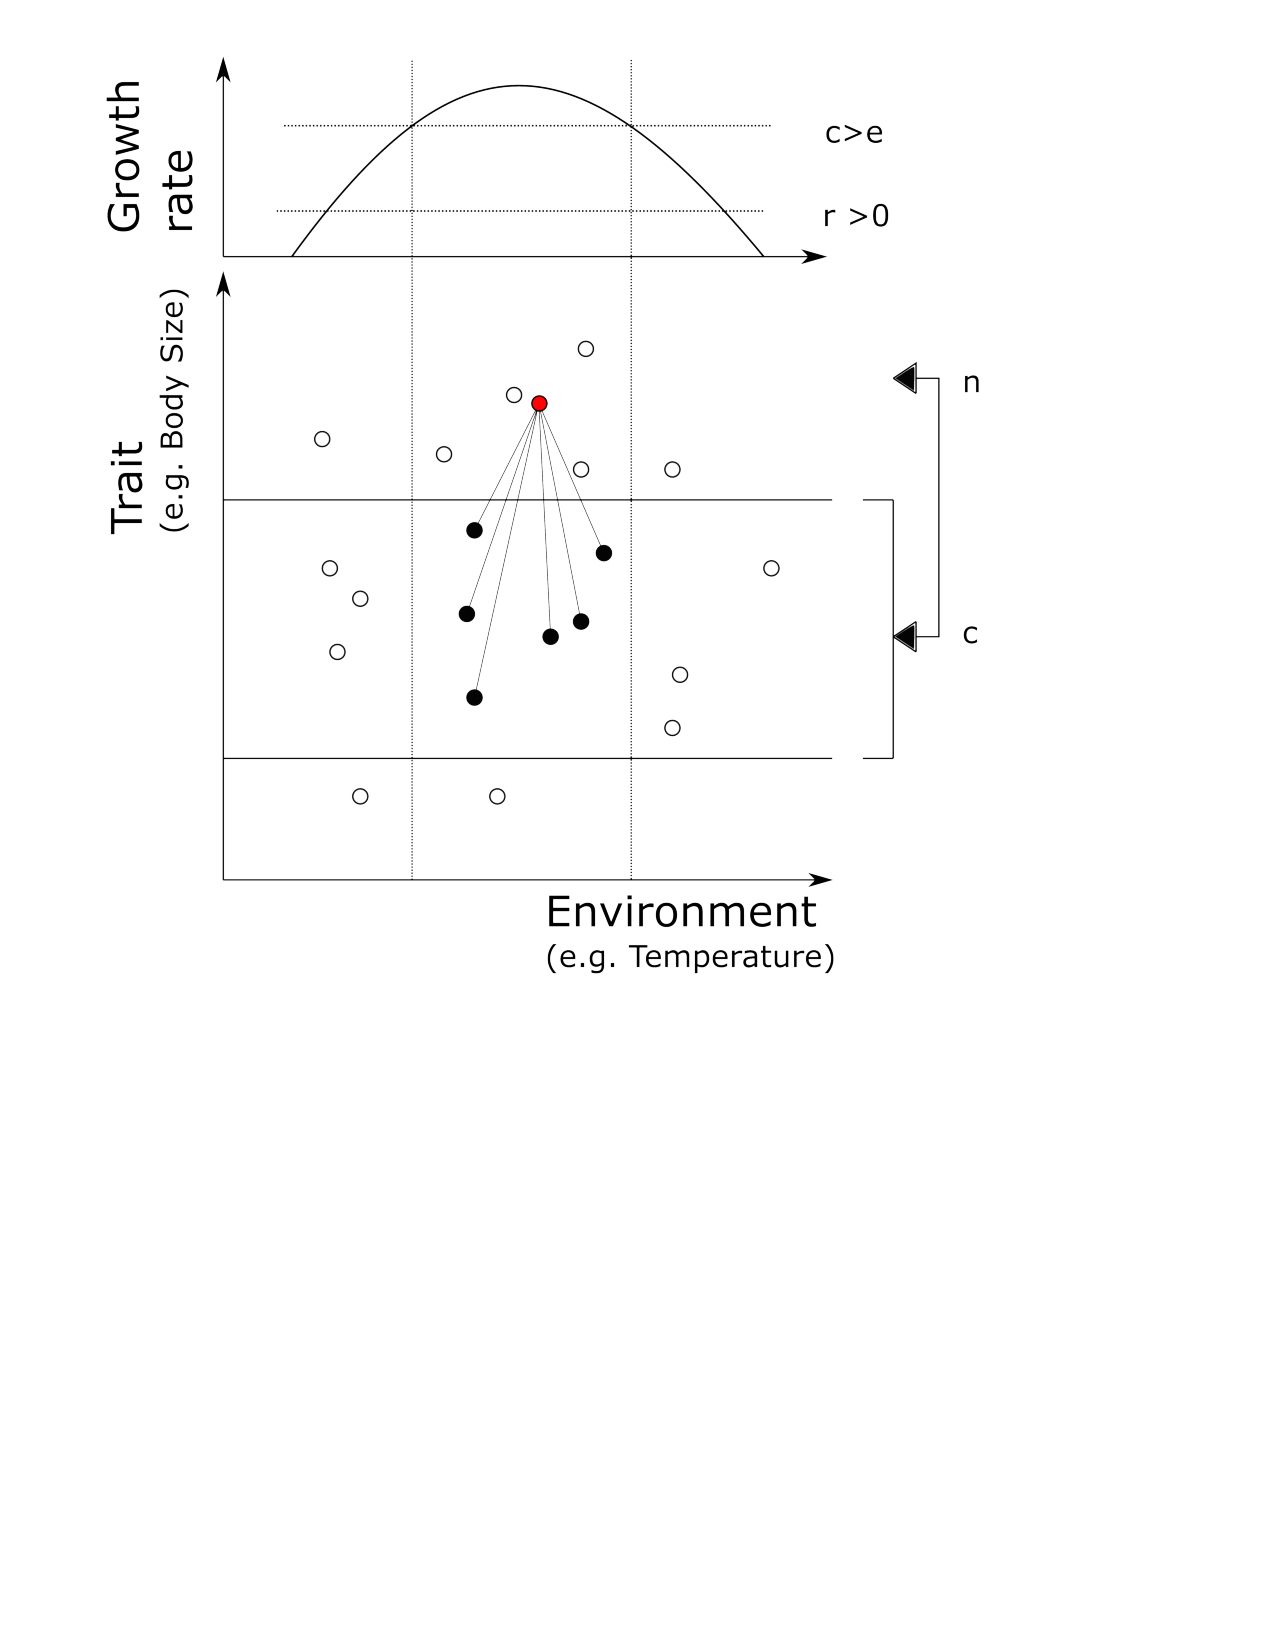
\includegraphics[width=0.8\textwidth]{niche}
\end{figure}

\newpage

%------------------------
\subsection*{Figure 3}

\begin{figure}[ht!]
	\centering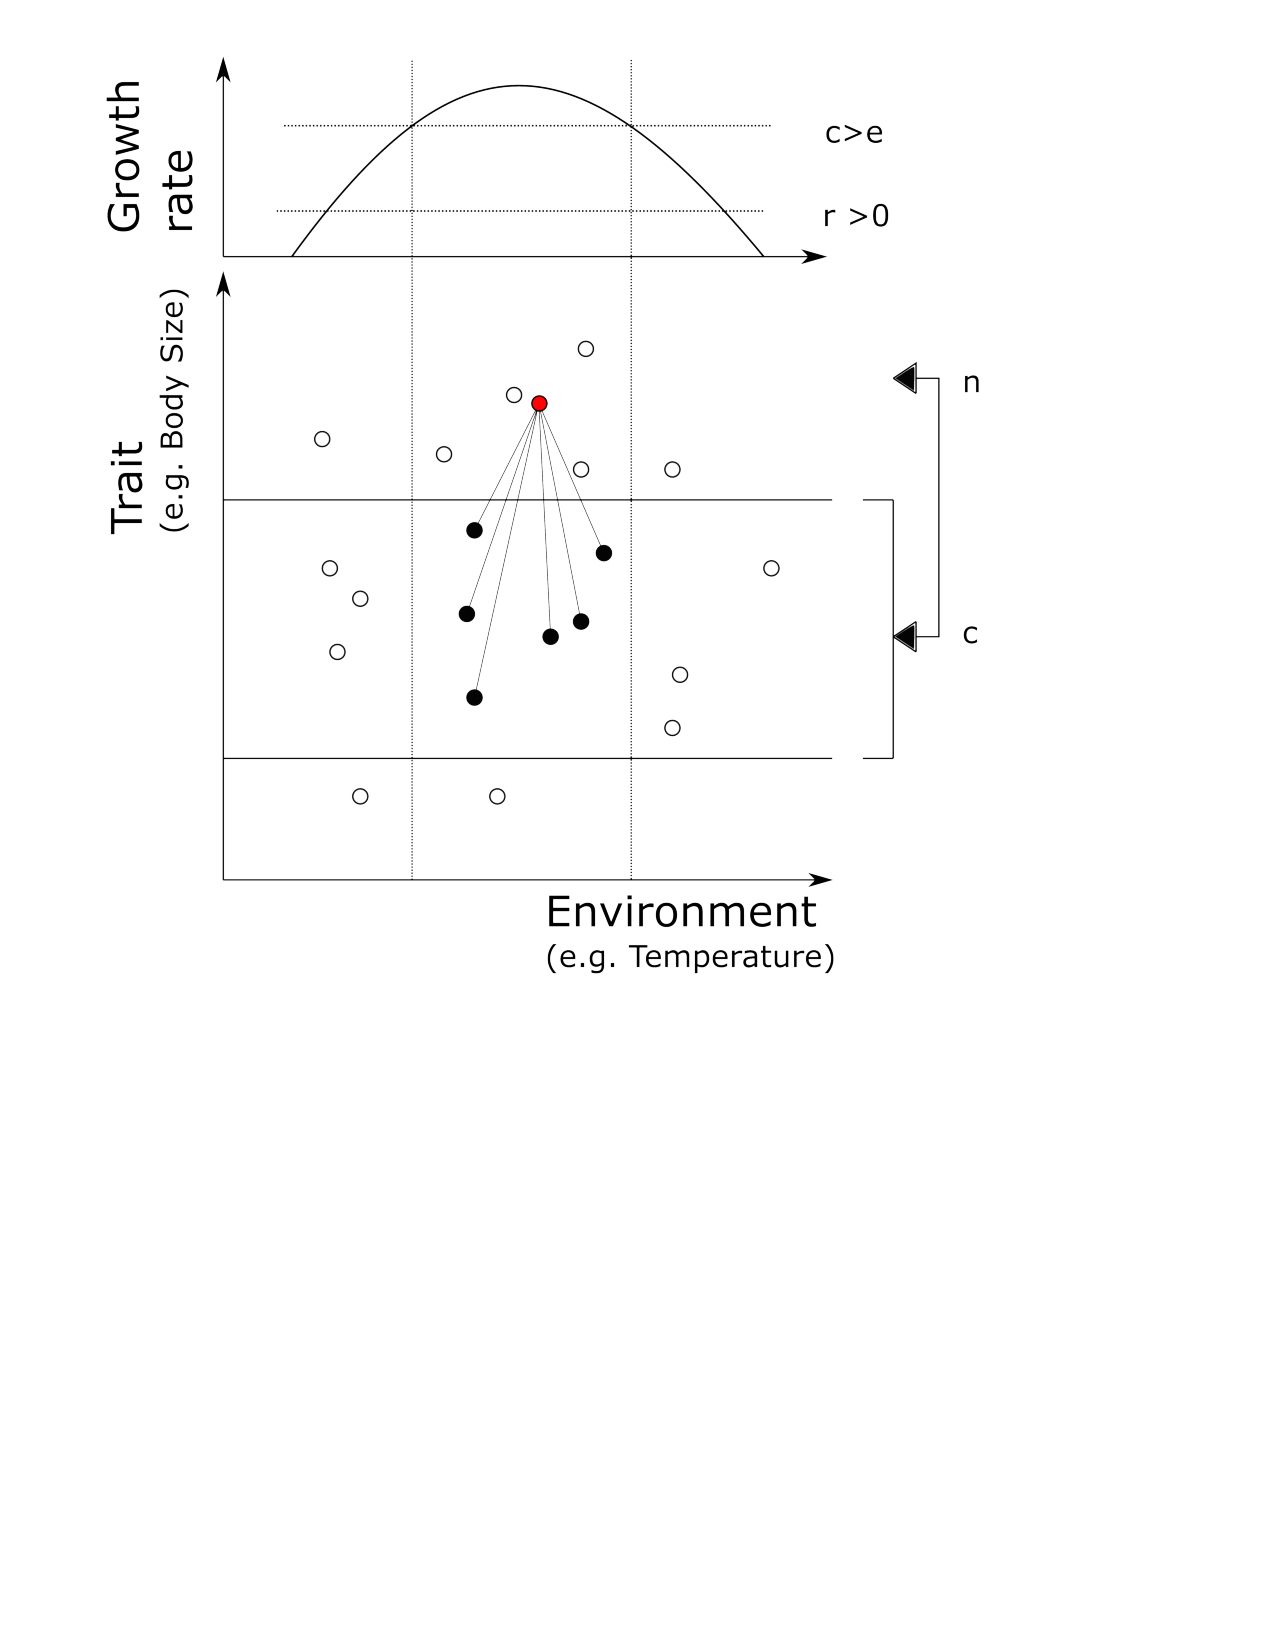
\includegraphics[width=0.8\textwidth]{niche}
\end{figure}

\newpage

%========================================================%

%------------------------
\begin{table*}[c]
	\centering
	\begin{tabular}{p{4cm}p{4cm}p{6cm}}
	\hline
	Name & Equation & Details \\
	\hline
	\textbf{Metaweb} &   &  \\
	Constant & $P(L_{ijy}|X_{iy},X_{jy})$ & Interaction probability is invariant to the environment \\
	Conditional & $P(L_{ijy}|X_{iy},X_{jy},E_y)$ & Interaction probability is a function of the local environment \\
	Deterministic & $P(L^*_{ijy}|X_{iy},X_{jy})$ & Interaction occurs whenever both species are present \\

	\textbf{Co-occurrence} & &\\
	Constant & $P(X_{iy},X_{jy})$ & Species distribution independent of $E$ \\
	Conditional on $E$ & $P(X_{iy},X_{jy} |E_y)$ & Similar to a SDM applied to co-occurrence \\
	Neutral & $P(X_{ix}|E_y)P(X_{jy}|E_y)$ & Independent SDMs fit to both species; could be independent of $E$ \\
	Conditional on $L_y$ & $P(X_{iy},X_{jy} | L_y)$ & Could account for first and higher order interactions \\
	\hline
	\end{tabular}
	\caption{List of different models}
\end{table*}

\newpage

%------------------------

\begin{sidewaystable}[c]
	\centering
	\begin{tabular}{lllllllll}
	\hline
	\textbf{Model} & \textbf{Metaweb} & & & \textbf{Co-occurrence} & & & \textbf{$L(H|D)$} & AIC\\
	 & Constant & Cond. on $E$ & Deterministic & Constant & Cond. on $E$ & Neutral & & \\
	\hline
	1. & X & & &  & X & & 0 & 0 \\
	2. & & X & &  & X & & 0 & 0 \\
	3. & &  & X & & X & & 0 & 0 \\
	4. & & X & & X & & & 0 & 0 \\
	5. & & X & & & X & & 0 & 0 \\
	6. & & X & & & & X & 0 & 0 \\
	\hline
	\end{tabular}
	\caption{Model comparison with the host-parasitoid networks. The 48 networks were fitted to different models of interaction networks. Note that for the computation of the likelihood all null interaction probabilities, co-occurrences and the pairwise interactions without observed co-occurrences were removed.
}
\end{sidewaystable}

\newpage

\end{document}
%========================================================%
